\scanpage{136}
Sur $\widetilde X^{\swarrow\!\searrow}$, il y a les opérations
$\sigma_1,\sigma,\sigma_2,\sigma_0$ dont deux consécutifs commutent.
\figure{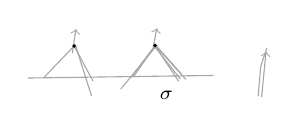
\begin{tikzpicture}[x=.55cm,y=-.55cm,line cap=round,line join=round,g/.style={olive!80!yellow,line width=1.7pt},r/.style={orange!80!brown,line width=1.8pt},w/.style={red!60!black,line width=1.5pt},b/.style={blue!60!black,line width=1.4pt},p/.style={gray!70,thin},k/.style={black,line width=1.2pt},every node/.style={font=\scriptsize}]
\draw[p] (17.98,1.73)--(22.25,1.67);
\draw[p] (18.34,1.72)--(19.04,.99)--(19.47,1.79);
\draw[p] (20.35,1.72)--(20.91,.98)--(21.62,1.76);
\draw[p] (20.12,1.98)--(20.91,1.02)--(21.49,1.75);
\draw[p] (20.41,1.7)--(20.92,.97)--(21.52,1.64);
\draw[p,->] (19.0,1.15)--(19.08,.6);
\draw[p,->] (20.86,1.05)--(20.95,.58);
\draw[p,->] (23.37,2.16)--(23.47,1.12);
\draw[p] (19.07,.97)--(19.44,2.14);
\draw[p] (20.92,1.0)--(21.45,1.8);
\draw[p] (23.29,2.14)--(23.35,1.45)--(23.49,1.04);
\fill[black] (19.04,.99) circle (.045);
\fill[black] (20.91,.98) circle (.045);
\node at (21.17,2.12) {$\unsure{\sigma}$};
\end{tikzpicture}}
\uline{faces de $\widetilde X$} : p.r. stables ; \uline{faces orientées} : p.r. orientées stables

\uline{arêtes de $\widetilde X$} : p.r. semi-stables ; \deleted{arêtes biorientées}

\uline{arêtes biorientées} i.e. repères : \deleted{\unsure{drapeaux}}\inserted{repères}
\[(D,s,\omega\inserted{,\bar\omega})\quad\text{où}\quad\left|\begin{array}{l}
D\text{ p.r. critique}\\
s\in S_D=D\cap S\\
\omega\text{ orientation de }D,\ \bar\omega\text{ ori. de }X\text{ en }s
\end{array}\right.\]
\inserted{ou \uline{repères}}
\[\text{i.e.}\quad\text{\unsure{Donc|Donner} \uline{repère p.r. :}}\quad(\unsure{D},S_D),+\]

\uline{Sommets} \deleted{$\unsure{\varphi}$} : \uline{p.r. critiques}

\uline{Sommets orientés} : p.r. \uline{orientées} critiques

\diagram{\[\begin{tikzcd}[ampersand replacement=\&,column sep=large]
\underset{\unsure{\varepsilon}}{\text{repères}}\arrow[r]\&\text{faces orientées}
\end{tikzcd}\]}
\[\deleted{\unsure{D}}(D,s,\omega)\longmapsto\text{la position relative stable obtenue en }\deleted{\text{\unsure{mouvant}}}\]
\margin{\mspage{135}}
